\subsubsection{Properties of $\pi \colon \Bx \to \Brx$}

In the previous section we have seen that similar to the symmetric case a 
functor into $\Brx$ satisfying the op-fibration condition and Segal condition
induces a braided monoidal structure on the fiber category over $\langle 1
\rangle$. However, for a colored braided operad $\B$, the forgetful functor
\[
    \pi \colon \Bx \to \Brx
\]
does not satisfy the op-fibration condition in general. 

In this section,
we investigate the properties of the forgetful functor $\pi$. Furthermore, we
see how to reconstruct the structure of a colored braided operad from such a
functor fulfilling these properties. This reconstruction together with the construction developing the forgetful functor $\pi$
then finally induces an equivalence, thus verifying that colored braided operads can indeed be formulated
in a categorical framework.

\begin{defin}
    A morphism $\alpha \colon \langle n \rangle \to  \langle m \rangle$ in
    $\Brx$ is called inert if it is inert in $\Fin$, i.e. for every $i \in
    \langle m \rangle^{\circ}$ the preimage $\alpha^{-1}(i)$ has exactly one
    element.
\end{defin}

\begin{eg}\label{eg:rho_i} For $n \in \N$ and $1 \leq i \leq n$, write $\rho^i$
    for the following inert morphism in $\Brx$:
    \begin{align*}
        \rho^i \colon \langle n \rangle &\to  \langle 1 \rangle \\
        \rho^i (j) &= 
        \begin{cases}
            1 & i=j \\
            * & \text{else},
        \end{cases}
    \end{align*}
    together with $\id^{(i)}$. 
\end{eg}



\begin{prop}\label{prop:Bx-fib-properties} Let $\B$ be a colored braided operad.
    The forgetful functor
    \[
        \pi \colon \Bx \to \Brx
    \]
    has the following properties:
    \begin{enumerate}
        \item For every inert morphism $\widetilde{\alpha} \colon \langle n
        \rangle \to \langle m \rangle$  in $\Brx$ and object $X \in \Bx$ there
        exists a $\pi$-cocartesian morphism $f \colon X \to X'$ lifting
        $\widetilde{\alpha}$ . In particular $\widetilde{\alpha}$ induces a
        functor 
        $$\pi_{\widetilde{\alpha}} \colon \Bx_{\langle n \rangle} \to
        \Bx_{\langle m \rangle}.$$
        \item For every pair of objects $X,Y$ in $\Bx$ the functor
        \[
                \Hom_{\Bx}(X,Y) \to \Hom_{\Brx}(\pi(X),\pi(Y))
        \]
        is a fibration.
        \item For a morphism $\widetilde{\alpha}$ in $\Brx$, the groupoid of
        morphisms lying over $\widetilde{\alpha}$:
        $$\Hom_{\D}^{\widetilde{\alpha}}(X, X')$$ is discrete. 
        \item Let $X = [X_1, \dots, X_n] \in \Bx_{\langle n \rangle}$ and $X' =
        [X_1', \dots, X_m'] \in \Bx_{\langle m \rangle}$ be objects, $\alpha :
        \langle n \rangle \to \langle m \rangle$ be a morphism in $\Brx$ and let
        $\Hom_{\Bx}^{\alpha}(X, X')$ be the set if morphisms over $\alpha$. 
        Choose $\pi$-cocartesian morphisms $X' \to X'_i$ lying over the inert
        morphism $\rho^i \colon \langle n \rangle \to \langle 1 \rangle$ for $1
        \leq i \leq n$. Then the induced map
        \[
            \Hom_{\Bx}^{\alpha}(X, X') \to \prod_{1 \leq i \leq n} \Hom_{\Bx}^{\rho^i \circ \alpha}(X, X_i')
        \]
        is an equivalence of groupoids. 
        
        \item For every finite collection of objects $X_1, \dots, X_n \in
        \Bx_{\langle 1 \rangle}$, there exists an object $X \in \Bx_{\langle n
        \rangle}$ and a collection of $p$-cocartesian morphism $X \to X_i$
        covering $\rho^i \colon \langle n \rangle \to \langle 1 \rangle$.
        % \item For all $n \in \N$, there is an equivalence of categories
        % \[
        %     \Bx_{\langle n \rangle} \cong \left(\Bx_{\langle 1 \rangle}\right)^n
        % \]
        % induced by the morphism $\rho^i$ from Example \ref{eg:rho_i}.
    \end{enumerate}
\end{prop}
% \todo{Reread proof}
\begin{proof}
    Let $B$ be a colored braided operad and $\pi \colon \Bx \to \Brx$ the above
    defined forgetful functor.
    \begin{enumerate}
        \item Let $\widetilde{\alpha} \colon \langle n \rangle \to  \langle m
        \rangle$ be an inert morphism in $\Brx$, i.e. for a restriction to the
        active subset of $\langle n \rangle$, there is a bijection of finite
        sets:
        \[
            \alpha \colon \alpha^{-1}(\langle m \rangle^{\circ}) \to \langle m \rangle^{\circ}
        \]
        and configurations $\widetilde{\alpha}_j \in \E_2(1)$ for all $j \in
        \langle m \rangle^{\circ}$. We denote $\alpha^{-1}(j) = \{\alpha_j\}$
        for all $1 \leq j \leq m$. Further, let $[X_1, \dots, X_n]$ be an object
        in $\Bx$. Then, we define
        \[
            f \colon [X_1, \dots, X_n] \to [X_1', \dots, X_m']
        \]
        as follows:

        We set the underlying morphism $\widetilde{\alpha_f} =
        \widetilde{\alpha}$. Further, we define $X_j = X_{\alpha_j}$ and
        \[
            f_j \in \Mul_{\B}(\{X_{\alpha_j}\},X_{\alpha_j})
        \]
        to be the identity $f_j = \id_{X_{\alpha_j}}$. We need to verify that
        $f$ is in fact cocartesian. Let $g \colon [X_1, \dots, X_n] \to [Y_1,
        \dots, Y_l]$ with underlying morphism $\pi(g) = \widetilde{\beta}$ and
        the following diagram in $\Brx$:
            \begin{center}
            \begin{tikzpicture}
                % Define node positions
                \node (B) at (0, 2) {$\langle n \rangle$}; \node (C) at (3, 2)
                {$\langle m \rangle$}; \node (A) at (1.5, 0) {$\langle l
                \rangle$};
                
                % Draw arrows
                \draw[->] (B) -- (C) node[midway, above] {\small
                $\widetilde{\alpha}$}; \draw[->] (B) -- (A) node[midway, left]
                {\small $\widetilde{\beta}$}; \draw[->] (C) -- (A) node[midway,
                right] {\small $\widetilde{\omega}$};
                
                % Natural transformation arrow
                \node at (1.5, 1.2) {$\overset{\eta}{\Leftarrow}$};
                % \node[rotate=-40] at (1.5, 1.2) {$\Downarrow \eta$};
            \end{tikzpicture}
        \end{center}
        We define $\bar{f} \colon  [X_1', \dots, X_m'] \to [X_1'', \dots,
        X_l'']$ in the following. We set the underlying morphism
        $\widetilde{\alpha_{\bar{f}}} = \widetilde{\omega}$. We claim that  
        without loss of generality, we can assume that $\widetilde{\alpha}_j$ is
        the trivial configuration because of the following fact: For any
        configurations $c, c' \in \E_2(1)$ there is exactly one homotopy class
        of paths from $c$ to $c'$ because the unit disk is contractible.
        Therefore, if $\widetilde{\alpha}_j$ is not trivial then there is a
        canonical extension 
        \begin{center}
            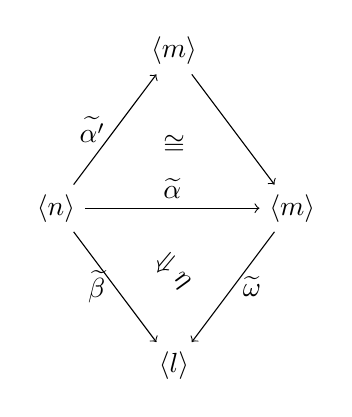
\begin{tikzpicture}
                % Define node positions
                \node (B) at (0, 2) {$\langle n \rangle$}; \node (C) at (3, 2)
                {$\langle m \rangle$}; \node (D) at (1.5, 4) {$\langle m
                \rangle$}; \node (A) at (1.5, 0) {$\langle l \rangle$};
                
                % Draw arrows
                \draw[->] (B) -- (C) node[midway, above] {$\widetilde{\alpha}$};
                \draw[->] (B) -- (A) node[midway, left] {$\widetilde{\beta}$};
                \draw[->] (C) -- (A) node[midway, right] {$\widetilde{\omega}$};
                \draw[->] (B) -- (D) node[midway, left] {$\widetilde{\alpha'}$};
                \draw[->] (D) -- (C) node[midway, right] {$\id$};
                
                % Natural transformation arrow
                \node[rotate=-40] at (1.5, 1.2) {$\Downarrow \eta$}; \node at
                (1.5, 2.8) {$\cong$};
                % \node at (1.7, 1.2) {$\eta$};
            \end{tikzpicture}
        \end{center}
        where $\widetilde{\alpha'}$ is $\alpha' = \alpha$ on finite pointed sets
        but equipped with the trivial collection of configurations
        $\{\id^{(\alpha_j)}\}_{j \in J}$. Hence, we gain $\widetilde{\omega}_k$ as
        a $\beta^{-1}(k)$-labeled configuration. The diagram in $\Br$ below:
        \begin{center}
            \begin{tikzpicture}
                % Define node positions
                \node (B) at (0, 2) {$(\omega \circ \alpha)^{-1}(k)$}; \node (C)
                at (3, 2) {$\beta^{-1}(k)$}; \node (A) at (1.5, 0) {$\{k\}$};
                
                % Draw arrows
                \draw[->] (B) -- (C) node[midway, above] {\small $\id$};
                \draw[->] (B) -- (A) node[midway, left] {\small
                $\widetilde{\omega}_k$}; \draw[->] (C) -- (A) node[midway,
                right] {\small $\widetilde{\beta}_k$};
                
                % Natural transformation arrow
                \node at (1.5, 1.2) {$\overset{\eta^{-1}}{\Leftarrow}$};
                % \node[rotate=-40] at (1.5, 1.2) {$\Downarrow \eta$};
            \end{tikzpicture}
        \end{center}
        gives a corresponding composition map in $\B$:
        $$
            \gamma \colon \prod_{p \in {\beta^{-1}(k)}} \Mul_{\B}^{\id^{(p)}}\left(\{X_{p}\}, X_{p}\right)\times \Mul_{\B}^{\widetilde{\beta}_k}\left(\{X_p\}_{p\in \beta^{-1}(k)}, Y_k\right) \to \Mul_{\B}^{\widetilde{\omega}_k} \left(\{X_{i_q}\}_{q \in \omega^{-1}(k)}, Y_k\right).
        $$
        We choose
        \[
            \bar{f}_k \coloneqq \gamma((\id_{X_p})_{p \in {\beta^{-1}(k)}}, g_k).
        \]
        Note that we obtain $g_k$, when we apply the composition, induced by 
        almost the same diagram but for
        $\eta$, to the morphism $\bar{f}_k$. This follows from the unitality
        property in $\B$ and is precisely why $\bar{f}_k$ can not be chosen
        differently. Hence, $\bar{f}$ is unique. 
        
        Furthermore, with this property the morphism $\widetilde{\alpha}$
        induces a functor of fibers
        \[
            \Bx_{\langle n \rangle} \to \Bx_{\langle m \rangle}
        \]
        sending
        \[
            [X_1, \dots, X_n] \mapsto [Y_1, \dots, Y_m]
        \]
        where $[Y_1, \dots, Y_m]$ corresponds to a cocartesian morphism $f
        \colon [X_1, \dots, X_n] \to [Y_1, \dots, Y_m]$ in $\Bx$. For a
        different choice of a cocartesian morphism $h \colon [X_1, \dots, X_n] \to
        [\bar{Y}_1, \dots, \bar{Y}_m]$ we obtain, due to the cocartesian
        property, two unique lifts $\bar{f}, \bar{h}$ that must be inverse to
        one another:
        \begin{center}
            \begin{tikzcd}
                {[X_1, \dots, X_n]} \arrow[rd, "h"'] \arrow[r, "f"] & { [Y_1,
                \dots, Y_m]} \arrow[d, "\bar{h}", dashed, shift left] &
                \rightarrow & \langle n \rangle \arrow[r, "\widetilde{\alpha}"]
                \arrow[rd, "\widetilde{\alpha}"'] & \langle m \rangle \\
                                                                    & {
                                                                    [\bar{Y}_1,
                                                                    \dots,
                                                                    \bar{Y}_m]}
                                                                    \arrow[u,
                                                                    "\bar{f}",
                                                                    dashed,
                                                                    shift left]
                                                                    & & &
                                                                    \langle m
                                                                    \rangle
                                                                    \arrow[u,
                                                                    "\id"']
            \end{tikzcd}
        \end{center}
        Hence, the functor is well-defined on objects up to unique isomorphism.
        For morphisms we define:
        \[
            (g \colon [X_1, \dots, X_n] \to [X_1', \dots, X_n'])  \mapsto (\bar{f} \colon [Y_1, \dots, Y_m] \to [Y_1', \dots, Y_m'])
        \]
        where $\bar{f}$ is the unique lift to the cartesian morphism $f$,
        corresponding to the following diagrams:
        \begin{center}
            \begin{tikzcd}
                {[X_1, \dots, X_n]} \arrow[r, "f!"] \arrow[d, "g"'] & {[Y_1,
                \dots, Y_m]} \arrow[d, "\bar{f}", dashed] & {} \arrow[r, "\pi",
                shift right=9] & {} & \langle n \rangle \arrow[d, "\id"]
                \arrow[r, "\widetilde{\alpha}"] & \langle m \rangle \arrow[d,
                "\id"] \\
                {[X_1', \dots, X_n']} \arrow[r, "f'!"]              & {[Y_1',
                \dots, Y_m']}                            & &    & \langle n
                \rangle \arrow[r, "\widetilde{\alpha}"]                  &
                \langle m \rangle                 
            \end{tikzcd}
        \end{center}


        The composition of two morphisms 
        \[
        g \colon [X_1, \dots, X_n] \to [X_1',
        \dots, X_n'], \; g' \colon [X_1', \dots, X_n'] \to [X_1'', \dots, X_n'']
        \]
        is being respected as the composition of the unique lifts $\bar{f}$ and
        $\bar{f}'$, lifts the diagram below and therefore have to be the unique lift for
        $g' \circ g$ and $f$:
        \begin{center}
            \begin{tikzcd}
                {[X_1, \dots, X_n]} \arrow[r, "!f"] \arrow[d, "g"']     & {[Y_1,
                \dots, Y_m]} \arrow[d, "\bar{f}", dashed] \\
                {[X_1', \dots, X_n']} \arrow[r, "!f'"] \arrow[d, "g'"'] &
                {[Y_1', \dots, Y_m']} \arrow[d, "\bar{f}'", dashed]      \\
                {[X_1'', \dots, X_n'']} \arrow[r, "!f''"']              &
                {[Y_1'', \dots, Y_m'']}                         
            \end{tikzcd}
        \end{center}
        \item Let $\phi \colon [X_1, \dots, X_n] \to [Y_1, \dots, Y_m]$ be a
        morphism in $\Bx$ with $\pi(\phi)=\alpha_{\phi}$ and $\widetilde{\eta} \colon
        \alpha_{\phi} \Rightarrow \alpha$ a $2$-morphism in $\Brx$. Then, we
        define a lift
        \[
            \psi \colon [X_1, \dots, X_n] \to [Y_1, \dots, Y_m]
        \]
        as follows: The underlying morphism we chose to be
        $\alpha_{\psi}=\alpha$. Furthermore, the $2$-morphism $\widetilde{\eta}$ gives rise
        to the following diagram in $\Br$:
        \begin{center}
            \begin{tikzpicture}
                % Define node positions
                \node (B) at (0, 2) {$\alpha_{\psi_j}$}; \node (C) at (3, 2)
                {$\alpha_{\phi_j}$}; \node (A) at (1.5, 0) {$\{j\}$};
                
                % Draw arrows
                \draw[->] (B) -- (C) node[midway, above] {\small $\id$};
                \draw[->] (B) -- (A) node[midway, left] {\small
                $\widetilde{\alpha_{\psi_j}}$}; \draw[->] (C) -- (A)
                node[midway, right] {\small $\widetilde{\alpha_{\phi_j}}$};
                
                % Natural transformation arrow
                \node at (1.5, 1.2) {$\overset{\widetilde{\eta_j}}{\Leftarrow}$};
                % \node[rotate=-40] at (1.5, 1.2) {$\Downarrow \eta$};
            \end{tikzpicture}
        \end{center}
        Then consider the corresponding composition map in $\B$:
        \[
            \gamma \colon \prod_{i \in \alpha_{\phi_j}} \Mul_{\B}^{\id^{(i)}}\left(\{X_i\}, X_i\right) \times \Mul_{\B}^{\widetilde{\alpha_{\phi_j}}}\left(\{X_i\}_{i \in \alpha_{\phi_j}}, Y_j\right) \to \Mul_{\B}^{\widetilde{\alpha_{\psi_j}}}\left(\{X_i\}_{i \in \alpha_{\psi_j}}, Y_j\right)
        \]
        We define
        \[
            \psi_j \coloneqq \gamma\left((\id_{X_i})_{i \in \alpha_{\psi_j}}, \phi_j\right).
        \]
        Thus, this constructs a $2$-morphism $\bar{\eta} \colon \phi \to \psi$ such that $\pi(\bar{\eta}) = \widetilde{\eta}$.
        Note, that with the same construction for $\widetilde{\eta}^{-1}$, we obtain $\bar{\eta}^{-1}$.
        % Let $\epsilon \colon \chi \Rightarrow \psi$ be another $2$-morphism in
        % $\Bx$ and $\widetilde{\delta}$ $2$-morphism in $\Brx$ such that
        % $\widetilde{\eta} \circ \delta = \widetilde{\epsilon}$. Note, that the
        % following hold for all $1 \leq j \leq m$:
        % \[
        %     \gamma((\id_{X_i})_{i \in \alpha_{\phi_j}}, \phi_j) = \psi_j = \gamma((\id_{X_i})_{i \in \alpha_{\chi_j}}, \chi_j)
        % \]
        % Then for the composition map for $\eta_j^{-1}$ together with the
        % associativity and unitality condition in $\B$ we obtain:
        % \begin{align*} \phi_j &= \gamma ((\id_{X_i})_{i \in \alpha_{\psi_j}},
        % \psi_j) \\
        %     &= \gamma((\id_{X_i})_{i \in \alpha_{\psi_j}}, (\id_{X_i})_{i \in
        %     \alpha_{\chi_j}}, \chi_j) \\
        %     &= ((\id_{X_i})_{i \in \alpha_{\chi_j}}, \chi_j) \end{align*} So,
        % $\epsilon = \eta^{-1} \circ \chi$ can be lifted to a $2$-morphism in
        % $\Bx$. \item The third property follows immediately from the
        % construction on $\Bx$. Since for morphisms $\phi, \psi \colon [X_1,
        % \dots, X_n] \to [Y_1, \dots, Y_m]$ a $2$-morphism $\eta \colon \phi
        % \to \psi$ with underlying $2$-morphism $\widetilde{\eta}$ is defined
        % by $\widetilde{\eta}_j$ for all $1 \leq j \leq m$. \item For $n \in
        % \N$, $1 \leq i \leq n$, the inert morphism
        % \[
        %     \rho^i \langle n \rangle \to \langle 1 \rangle,
        % \]
        % as defined in \ref{eg:rho_i}, induces a functor on fiber categories:
        % \[
        %     P^i \colon \Bx_{\langle n \rangle} \to \Bx_{\langle 1 \rangle}.
        % \]
        % Thus,
        % \[
        %     \prod_{1 \leq i \leq n} P^i \colon \Bx_{\langle n \rangle} \to \left(\Bx_{\langle 1 \rangle}\right)^n
        % \]
        % is fully faithful and essentially surjective. This follows immediately
        % when considering the construction of $P^i$.
        \item[3. + 4.] This follows immediately by construction of $\Bx$ and the
        unitality condition in $\B$.
        \item[5.] By construction of $\Bx$ the following holds: For $X_1, \dots,
        X_n$ colors in $\B$ the morphism
        \[
            \phi \colon [X_1, \dots, X_n] \to [X_i]
        \]
        with $\rho^i$ and $\phi_i = \id_{X_i}$ covers $\rho^i$ for all $1 \leq i
        \leq n$.
    \end{enumerate}
\end{proof}

The Corollary in \cite[Corollary 2.4.6.5]{hht} gives a definition of a
categorical fibration for simplicial sets. For a functor of $\Grp$-enriched
categories this breaks down to the following definition:
%  the following notion of categorical fibrations:
% \begin{defin}\label{def:cat-fib-infty} Let $p \colon \C \to \D$ be a map of
% simplicial sets, where $\D$ is an $\infty$-category. We call $p$ a categorical
% fibration if the following conditions hold: \begin{enumerate}[(i)] \item The
% map $p$ is an inner fibration as defined in
% \cite[\href{https://kerodon.net/tag/01BA}{Definition 01BA}]{kerodon}, i.e.
% every lifting problem for $0 < i < n$: \begin{center} \begin{tikzcd}
% \Lambda_i^n \arrow[r] \arrow[d]       & \C \arrow[d] \\
%                 \Delta^n \arrow[r] \arrow[ru, dashed] & \D          
%             \end{tikzcd} \end{center}

%         admits a solution.
%         \item For every equivalence $f \colon D \to D'$ in $\D$ and every object
%         $C \in \C$ with $p(C) = D$, there exists an equivalence $\bar{f} \colon
%         C \to C'$ in $\C$ with $p(\bar{f}) = f$.
%     \end{enumerate}
% \end{defin}

\begin{defin}\label{def:cat-fib-grpd} Let $p \colon \C \to \D$ be a functor of
    $\Grp$-enriched category. We call $p$ a categorical fibration if the
    following conditions hold:
    \begin{enumerate}[(i)]
        % \item The map $p$ is an inner fibration as defined in
        % \cite[\href{https://kerodon.net/tag/01BA}{Definition 01BA}]{kerodon},
        % i.e. every lifting problem for $0 < i < n$: \begin{center}
        % \begin{tikzcd} \Lambda_i^n \arrow[r] \arrow[d]       & \C \arrow[d] \\
        %         \Delta^n \arrow[r] \arrow[ru, dashed] & \D          
        %     \end{tikzcd} \end{center}

        % admits a solution.
        \item For every pair of objects $X,Y$ in $\C$ the functor
        \[
            p \colon \Hom_{\C}(X,Y) \to \Hom_{\D}(p(X), p(Y))
        \]
        is a fibration.
        \item For every equivalence $f \colon D \to D'$ in $\D$ and every object
        $C \in \C$ with $p(C) = D$, there exists an equivalence $\bar{f} \colon
        C \to C'$ in $\C$ with $p(\bar{f}) = f$.
    \end{enumerate}
\end{defin}

\begin{rem}
    Note that an equivalence $\widetilde{\alpha} \colon \langle n \rangle \to
    \langle m \rangle$ in $\Brx$ is in particular an inert morphism as the
    restriction to $\alpha^{-1}(\langle m \rangle^{\circ})$ is a bijection.
    Thus, in the proof of Proposition \ref{prop:Bx-fib-properties} the
    construction of the cocartesian lift of an inert morphism implies condition
    (ii) from Definition \ref{def:cat-fib-grpd} for the forgetful functor $\pi
    \colon \Bx \to \Brx$.
\end{rem}

\begin{defin}\label{def:operadicfib}
    An {\em operadic fibration} is a functor between $\Grp$-enriched categories
    \[
        \pi \colon \D \to \Brx
    \]
    satisfying the following conditions:
    \begin{enumerate}[(i)]
    \item The functor $\pi$ is a categorical fibration (c.f. Definition
    \ref{def:cat-fib-grpd}).
    \item For every inert morphism $\widetilde{\alpha} \colon \langle n \rangle
    \to \langle m \rangle$ in $\Brx$ and object $X \in \D$ there exists a
    $\pi$-cocartesian morphism $f \colon X \to X'$ lifting $\widetilde{\alpha}$. In
    particular, $\widetilde{\alpha}$ induces a functor: $$\pi_{\widetilde{\alpha}} \colon
    \Bx_{\langle n \rangle} \to \Bx_{\langle m \rangle}.$$
    \item For a morphism $\widetilde{\alpha}$ in $\Brx$, the groupoid of
    morphisms lying over $\widetilde{\alpha}$:
    $$\Hom_{\D}^{\widetilde{\alpha}}(X, X')$$ is discrete.
    \item Let $X \in \D_{\langle n \rangle}$ and $X' \in \D_{\langle m \rangle}$
    be objects, $\widetilde{\alpha}  : \langle n \rangle \to \langle m \rangle$
    be a morphism in $\Brx$ and let $$\Hom_{\D}^{\widetilde{\alpha}}(X, X')$$ be the 
    % isomorphism class of 
    morphisms which lie over $\widetilde{\alpha}$. 
    Choose $\pi$-cocartesian morphisms $X' \to X'_i$ lying over the inert
    morphism $\rho^i \colon \langle n \rangle \to \langle 1 \rangle$ for $1 \leq
    i \leq n$. Then the induced map
    \[
        \Hom_{\D}^{\widetilde{\alpha}}(X, X') \to \prod_{1 \leq i \leq n} \Hom_{\D}^{\rho^i \circ \widetilde{\alpha}}(X, X_i')
    \]
    is an equivalence of groupoids. 
    
    \item For every finite collection of objects $X_1, \dots, X_n \in
    \D_{\langle 1 \rangle}$, there exists an object $X \in \D_{\langle n
    \rangle}$ and a collection of $\pi$-cocartesian morphism $X \to X_i$
    covering $\rho^i \colon \langle n \rangle \to \langle 1 \rangle$.
    % \item For all $n \in \N$, there is an equivalence of categories
    % \[
    %     \Bx_{\langle n \rangle} \cong \left(\Bx_{\langle 1 \rangle}\right)^n
    % \]
    % induced by the morphism $\rho^i$ from Example \ref{eg:rho_i}.
    \end{enumerate}
\end{defin}





\begin{prop}
    Let
    \[
        \pi \colon \D \to \Brx
    \]
    be an operadic fibration over $\Brx$. Then we can reconstruct a colored
    braided operad $\B$ from $\D$ such that, $\D \cong \Bx$ and the functor
    \[
        \Bx \cong \D \overset{\pi}{\to} \Brx
    \]
    is the usual forgetful functor from $\Bx$ to $\Brx$.
\end{prop}
For this statement, we only sketch a reconstruction of a colored braided
operad. Defining the equivalence should then be straightforward by the
construction.

\begin{proof}
    Let
    \[
        \pi \colon \D \to \Brx
    \]
    be an operadic fibration. We define a colored braided operad $\B$ from
    $\D$ and $\pi$. The fiber category $\D_{\langle 1 \rangle}$ is the
    underlying category of $\B$. The objects in $\D_{\langle 1 \rangle}$ are the
    colors of $\B$. 
    
    Let $I$ be a finite set with $|I|=n$, $\widetilde{I} \in \E_2(n)$ an
    $I$-labeled configuration, $\{X_i\}_{i \in I}$ a collection of colors and
    $Y$ a color. A priori we choose a bijection $\iota \colon I \cong \langle n
    \rangle$ for every finite set $I$. 
    By (iii) we get that there is an object $X \in \D_{\langle n
    \rangle}$ and a collection of morphisms $X \to X_i$ covering $\rho^i$ for $i
    \in I$. Then, 
    \[
        \Mul_{\B}^{\widetilde{I}}\left(\{X_i\}_{i \in I}, Y\right)
    \]
    is the set of morphisms $f \colon X \to Y$ in $\D$ such that $\pi(f)$
    corresponds to the active morphism
    \[
        \langle n \rangle \to \langle 1 \rangle
    \]
    with configuration $\widetilde{I}$ in $\Brx$.
    For the following triangle in $\Br$:
            \begin{center}
            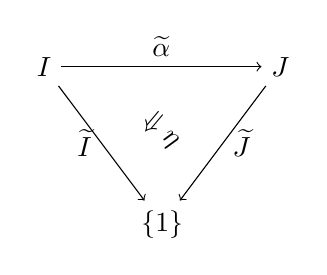
\begin{tikzpicture}
                % Define node positions
                \node (B) at (0, 2) {$I$}; \node (C) at (3, 2) {$J$}; \node (A)
                at (1.5, 0) {$\{ 1 \}$};
                
                % Draw arrows
                \draw[->] (B) -- (C) node[midway, above] {$\widetilde{\alpha}$};
                \draw[->] (B) -- (A) node[midway, left] {$\widetilde{I}$};
                \draw[->] (C) -- (A) node[midway, right] {$\widetilde{J}$};
                
                % Natural transformation arrow
                \node[rotate=-40] at (1.5, 1.2) {$\Downarrow \eta$};
                % \node at (1.7, 1.2) {$\eta$};
            \end{tikzpicture}
        \end{center}
    along with collections of colors $\{X_i\}_{i \in I}, \{Y_j\}_{j \in J}$ and
    color $Z$, we define a composition map via the composition in $\D$ as
    follows: Via the chosen bijections of $I \cong \langle n \rangle^{\circ}$, $J
    \cong \langle m \rangle^{\circ}$ we obtain the following diagram in $\Brx$:
    \begin{center}
        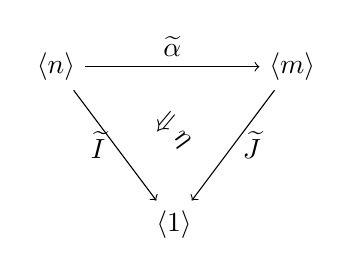
\begin{tikzpicture}
            % Define node positions
            \node (B) at (0, 2) {$\langle n \rangle$}; \node (C) at (3, 2)
            {$\langle m \rangle$}; \node (A) at (1.5, 0) {$\langle 1 \rangle$};
            
            % Draw arrows
            \draw[->] (B) -- (C) node[midway, above] {$\widetilde{\alpha}$};
            \draw[->] (B) -- (A) node[midway, left] {$\widetilde{I}$}; \draw[->]
            (C) -- (A) node[midway, right] {$\widetilde{J}$};
            
            % Natural transformation arrow
            \node[rotate=-40] at (1.5, 1.2) {$\Downarrow \eta$};
            % \node at (1.7, 1.2) {$\eta$};
        \end{tikzpicture}
    \end{center}
    where $\widetilde{I}$, $\widetilde{J}$, $\widetilde{\alpha}_j$ denote the
    corresponding configurations in $\E_2$ after identification via the
    bijections. Furthermore, note that by conditions (iv) and (v), for  colors
    $\{X_i\}_{i \in \alpha_j}$ there is an object $X^{(\alpha_j)}$ in
    $\D_{\langle |\alpha_j| \rangle}$ and coCartesian morphisms $X^{(\alpha_j)} \to X_i$
    covering $\rho^i$. For $\{X^{(\alpha_j)}\}_{1 \leq j \leq m}$ there is also
    an object X with morphisms $X \to X^{(\alpha_j)}$ covering $\rho^j$ for $1 \leq
    j \leq m$. We observe that $X$ with the composite morphism $X \to X_i$ covers
    $\rho^i$. We consider the following composition in $\D$:
    \[
       \theta \colon \prod_{1 \leq j \leq m} \Hom^{\rho^j}(X, X^{(\alpha_j)}) \times \Hom^{\widetilde{\alpha}_j}(X^{(\alpha_j)}, Y_j) \to \prod_{1 \leq j \leq m} \Hom^{\rho^j \circ \widetilde{\alpha}} (X, Y_j) \cong \Hom^{\widetilde{\alpha}}(X, Y)
    \]

    % \[
    % \prod_{\1 \leq j \leq m} \Hom^{\rho^j \circ \widetilde{\alpha}} (X, Y_j)
    % \cong \Hom^{\widetilde{\alpha}}(X, Y)
    % \]
    Let $\theta'$ be the restriction of $\theta$ to the covering morphisms $X
    \to X^{(\alpha_j)}$. The restriction to the image of $\theta'$ of the
    following composition map in $\D$
    \[
        \Hom^{\widetilde{\alpha}}(X, Y) \times \Hom^{\widetilde{J}}(Y, Z) \to \Hom^{\widetilde{I}}(X, Z)
    \]
    defines a composition map:
    \[
        \gamma \colon \prod_{j \in J} \Mul_{\B}^{\widetilde{\alpha}_j}(\{X_i\}_{i \in \alpha_j}, Y_j) \times \Mul_{\B}^{\widetilde{J}}(\{Y_j\}_{j \in J}, Z) \to \Mul_{\B}^{\widetilde{I}}(\{X_i\}_{i \in I}, Z).
    \]

    This construction is well-defined. 
    % When choosing covering morphisms $X \to
    % X_i$ for $\rho^i$ we can assume they are cocartesian lifts. If not, then
    % there is a cocartesian lift $X \to X_i'$ for $\rho^i$ and $X$ because of
    % property (ii). Then, there is a unique morphism $X_i' \to X_i$ lying over an
    % equivalence in $\Brx$. By (i), there is an equivalence $X_i' \cong X_i$ in
    % $\D$.
    % with morphisms $X \to X_$ covering $\rho^i$ for $1 \leq i \leq n$, as well
    % as an object $Y$ in $\D_{\langle m \rangle}$ with morphisms $Y \to Y_j$
    % covering $\rho^j$ for $1 \leq j \leq m$.
    The identity morphisms in $\B$ are given by the identity morphisms in the
    fiber category $\D_{\langle 1 \rangle}$, i.e. for each color $X \in
    \D_{\langle 1 \rangle}$, the identity morphism $\id_X$ in $\D$ defines the
    identity morphism in $\Mul_{\B}^{\id}(\{X\}, X)$. The associativity
    requirement is met as the composition is defined via the composition map in
    $\D$ which is associative. The unitality condition is also induced by the
    unitality in $\D$. This construction gives rise to an equivalence of
    categories $\Bx \cong \D$ such that the composition $\Bx \cong \D \to \Brx$
    is indeed the forgetful functor.
\end{proof}


